% !TEX root = BachelorBookletMain.tex

\chapter{Workflow}
In this project I fallowed an iterative prototype workflow, creating multiple prototypes to evaluate specific ideas. As for implementing different systems needed for the application, I followed the workflow of researching a single component\footnote{Such as the Kears functional API, UDP sockets, etc.} and then implementing it, before beginning further researching efforts.

What fallows is a description of the prototypes developed over the course of the project. The main prototype, called "maze game", became the focus of the project after the direction had been set with the help of the results obtained from previous prototypes. The maze game is described in detail in \cref{MazeGameSystems}.


\section{Functional}
The goal of the first prototype was to developed the core systems. The entire data generation- and preprocessing pipeline and the neural network model where implemented and evaluated. A small level with checkerboard textures was created for this prototype (\cref{FunctionalFirstPerson} and \cref{FunctionalCapture}). The sky and wall colors are variable between environments. An environment is a variation of a level. In this case, everything but the sky and wall colors stays constant for each environment, e.g. the walls are always at the same position in each environment. As \cref{FunctionalFirstPerson} shows, the network can adjust its output based on the information that is being fed in. The network is able to this without retraining. All that needs to be changed is the inputs to the encoder (\cref{GQNArchitectureGraph}). More information on the systems developed in this prototype can be found in \cref{NeuralNetworkSystems}.

\begin{figure}[p]
  \centering
  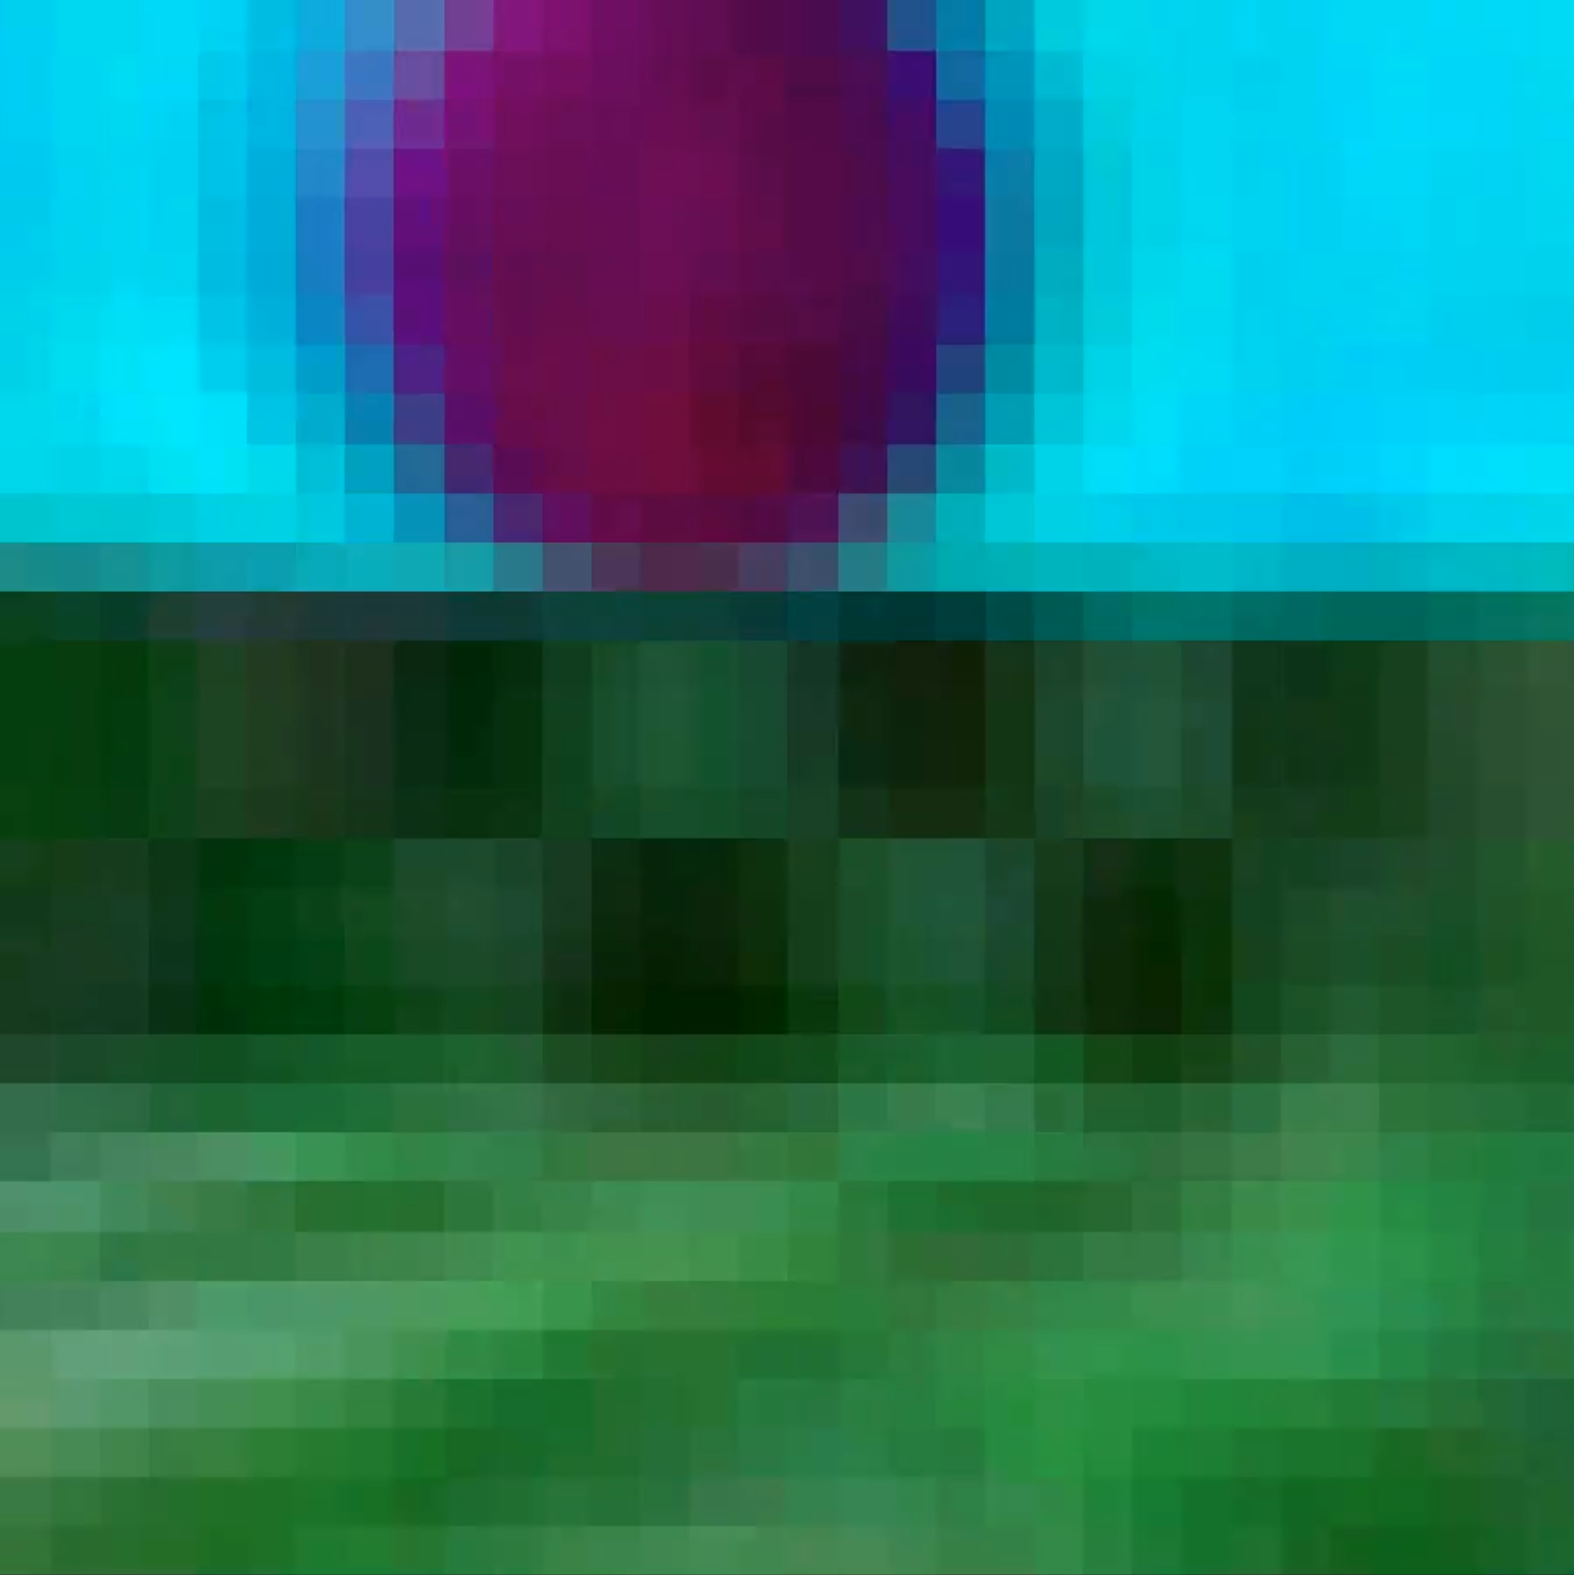
\includegraphics[height=\imgWithTripple]{images/workflow/FunctionalF1.png} \\[\picVdist]
  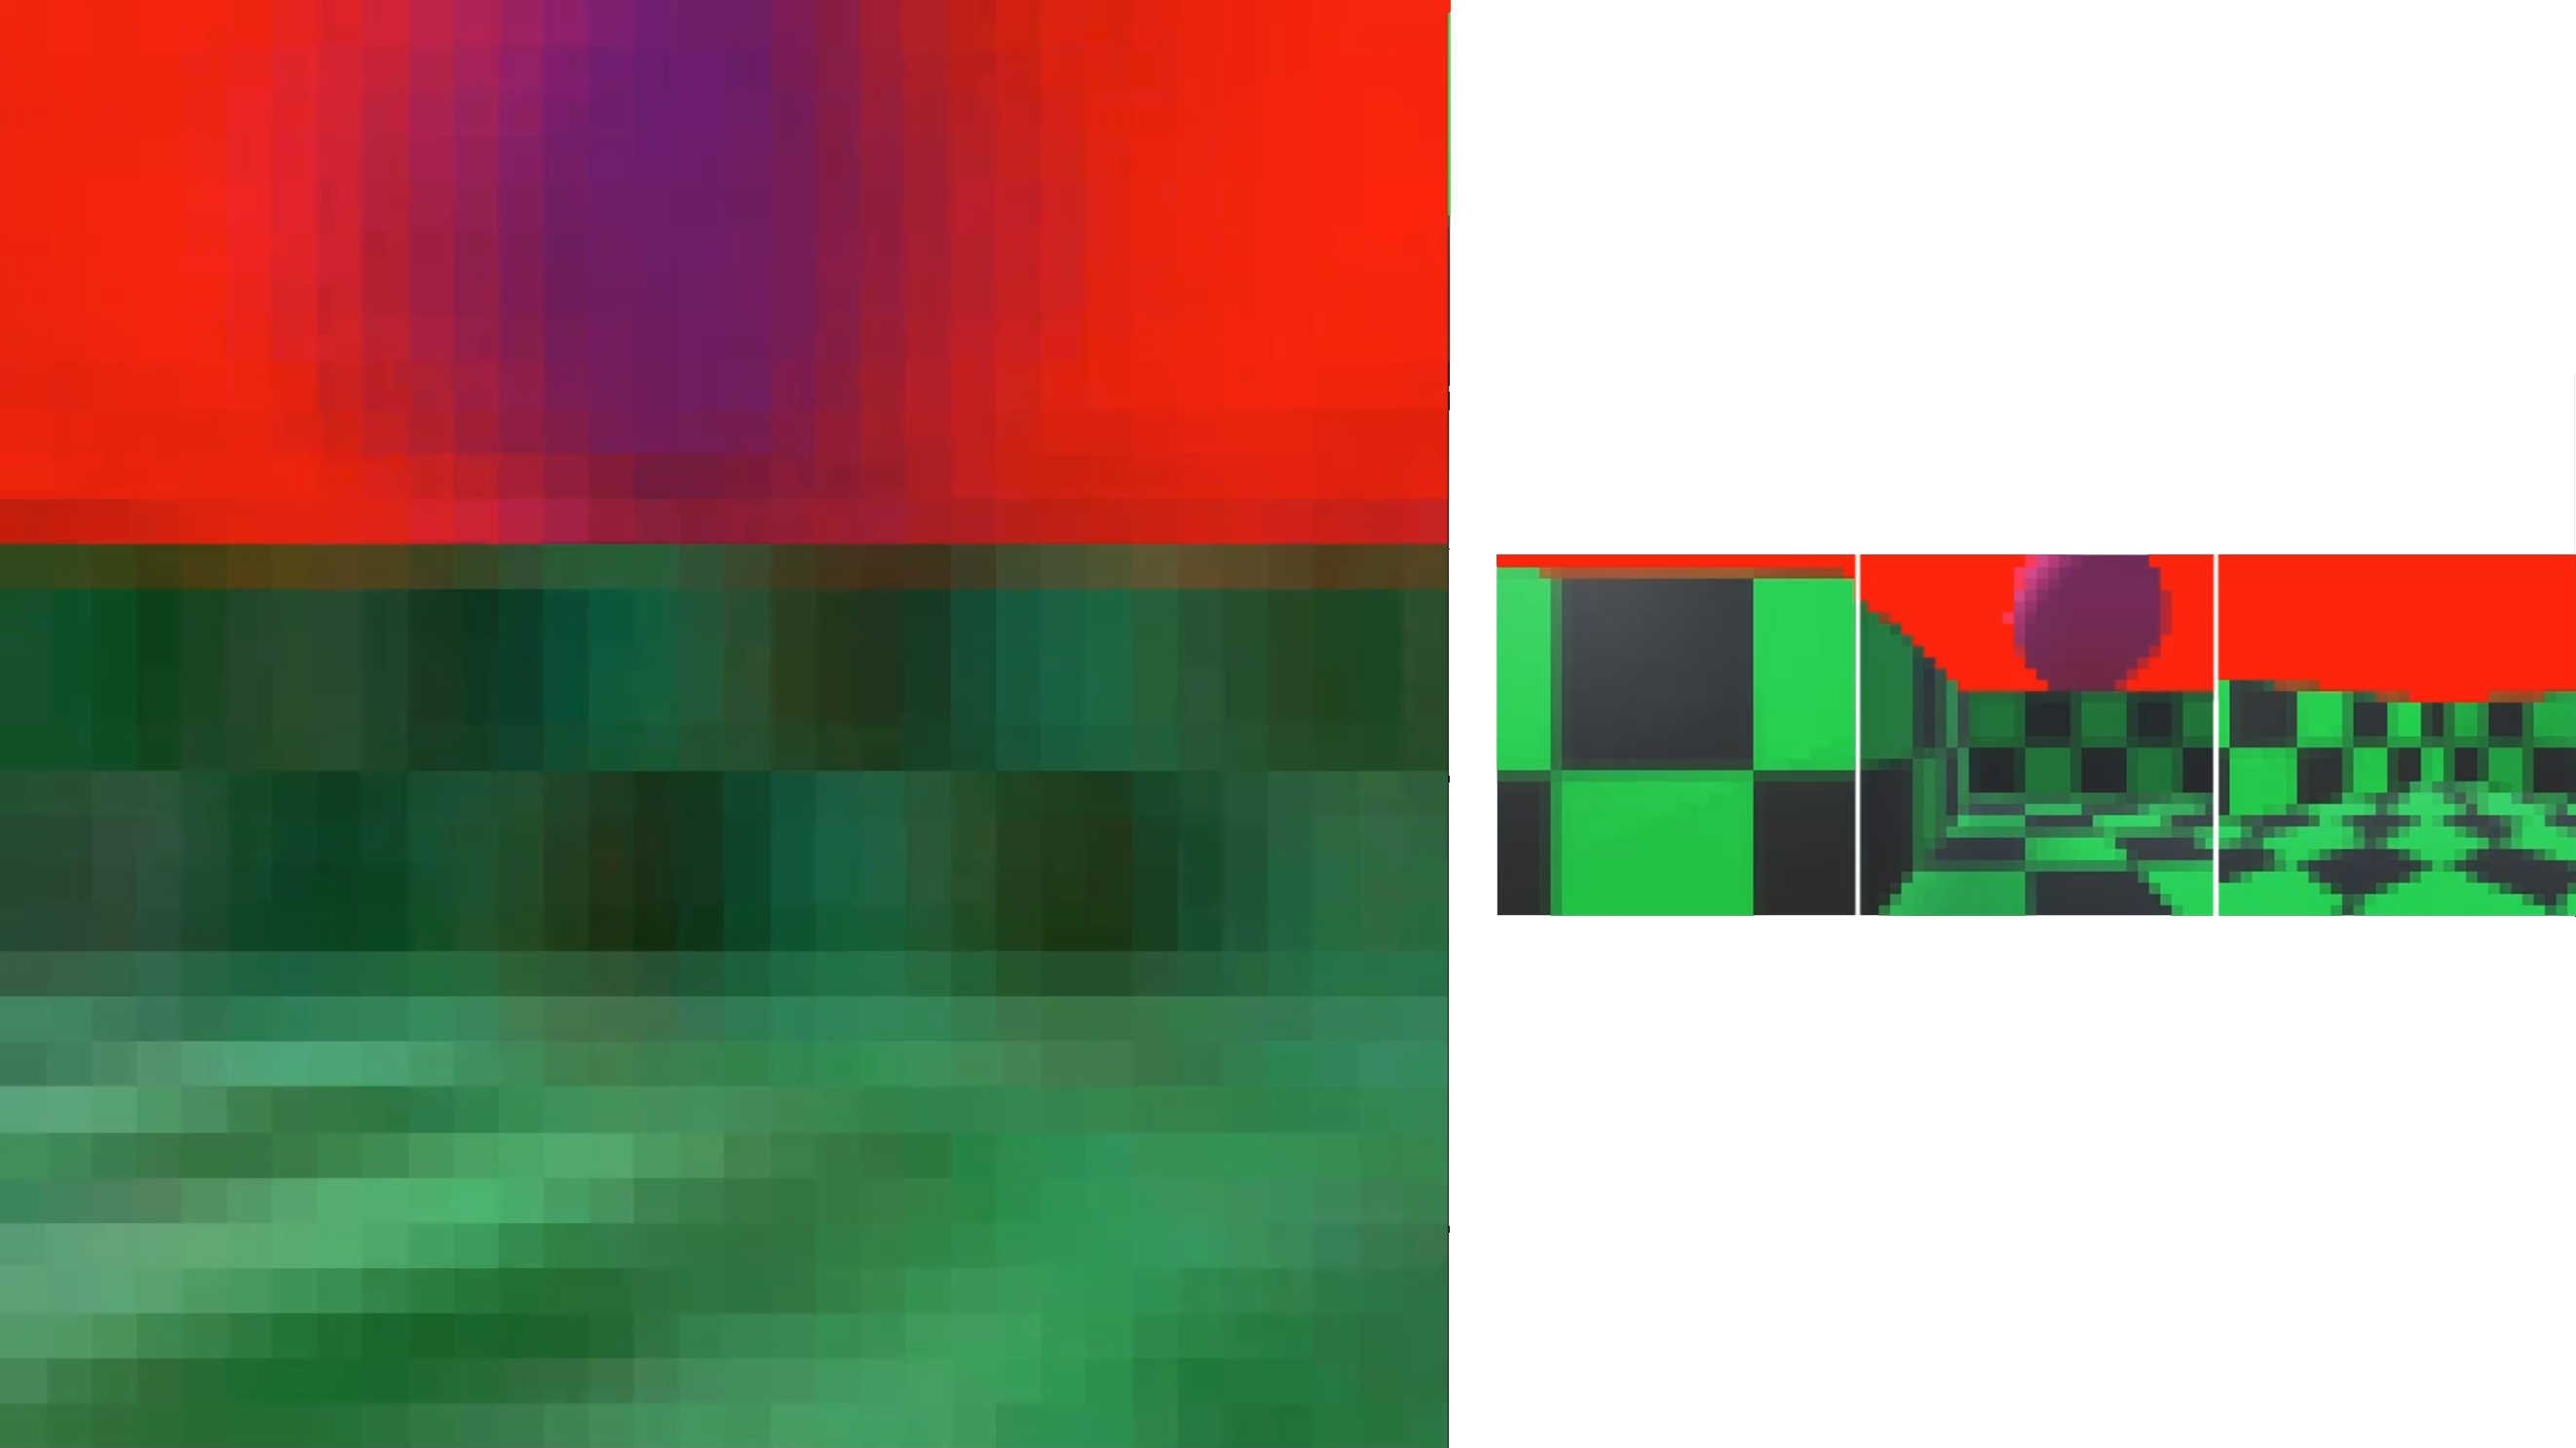
\includegraphics[height=\imgWithTripple]{images/workflow/FunctionalF2.png} \\[\picVdist]
  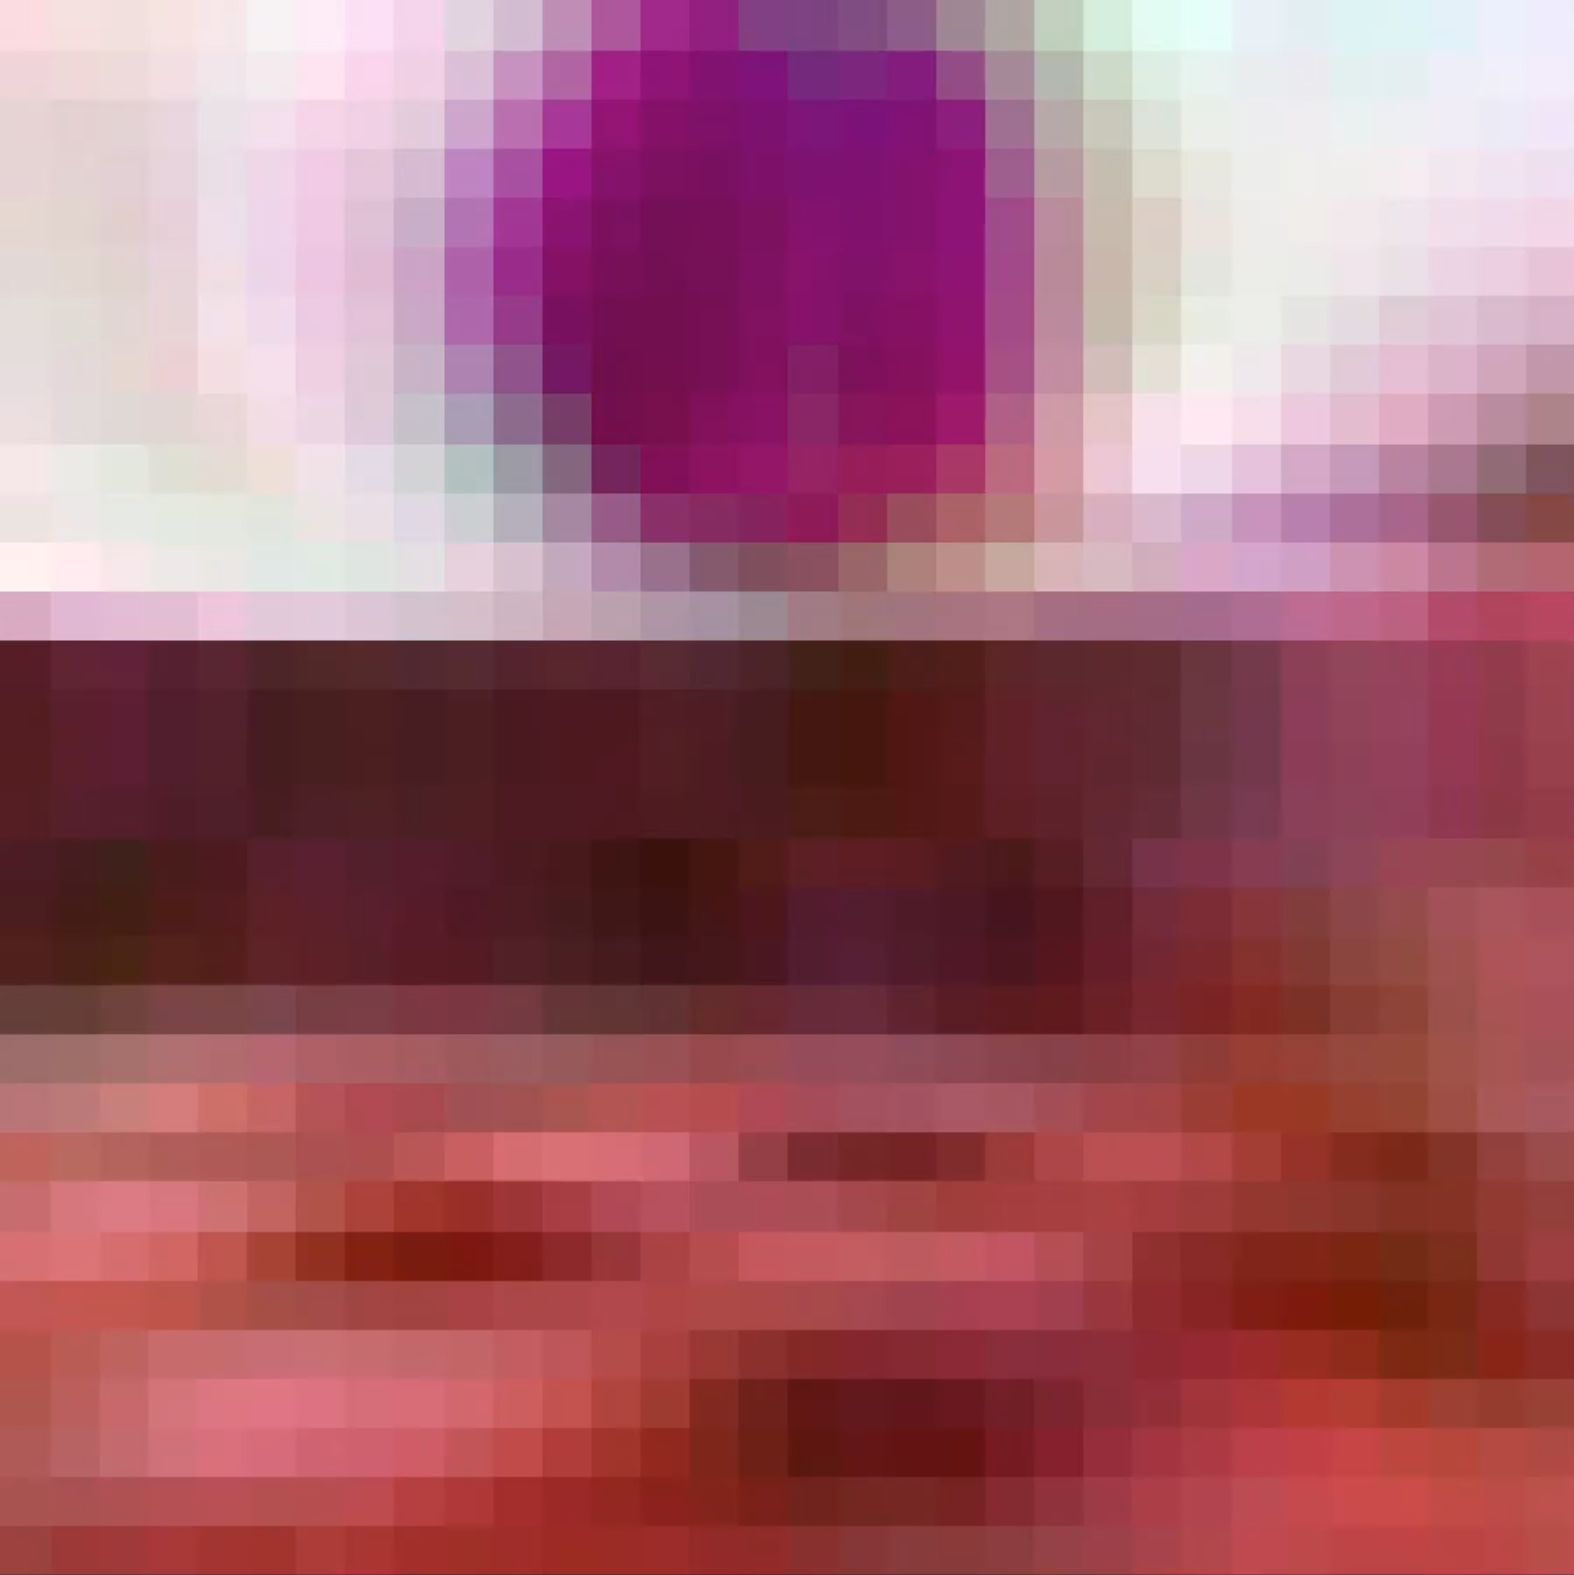
\includegraphics[height=\imgWithTripple]{images/workflow/FunctionalF3.png}
  \caption{The neural network predicts different colors based on the input data that makes up $R$. The input pictures are shown to the right. The network gives output even if no images are fed in as seen in the last image.}
  \label{FunctionalFirstPerson}
  \figsource{own graphic}
\end{figure}

\begin{figure}[p]
  \centering
  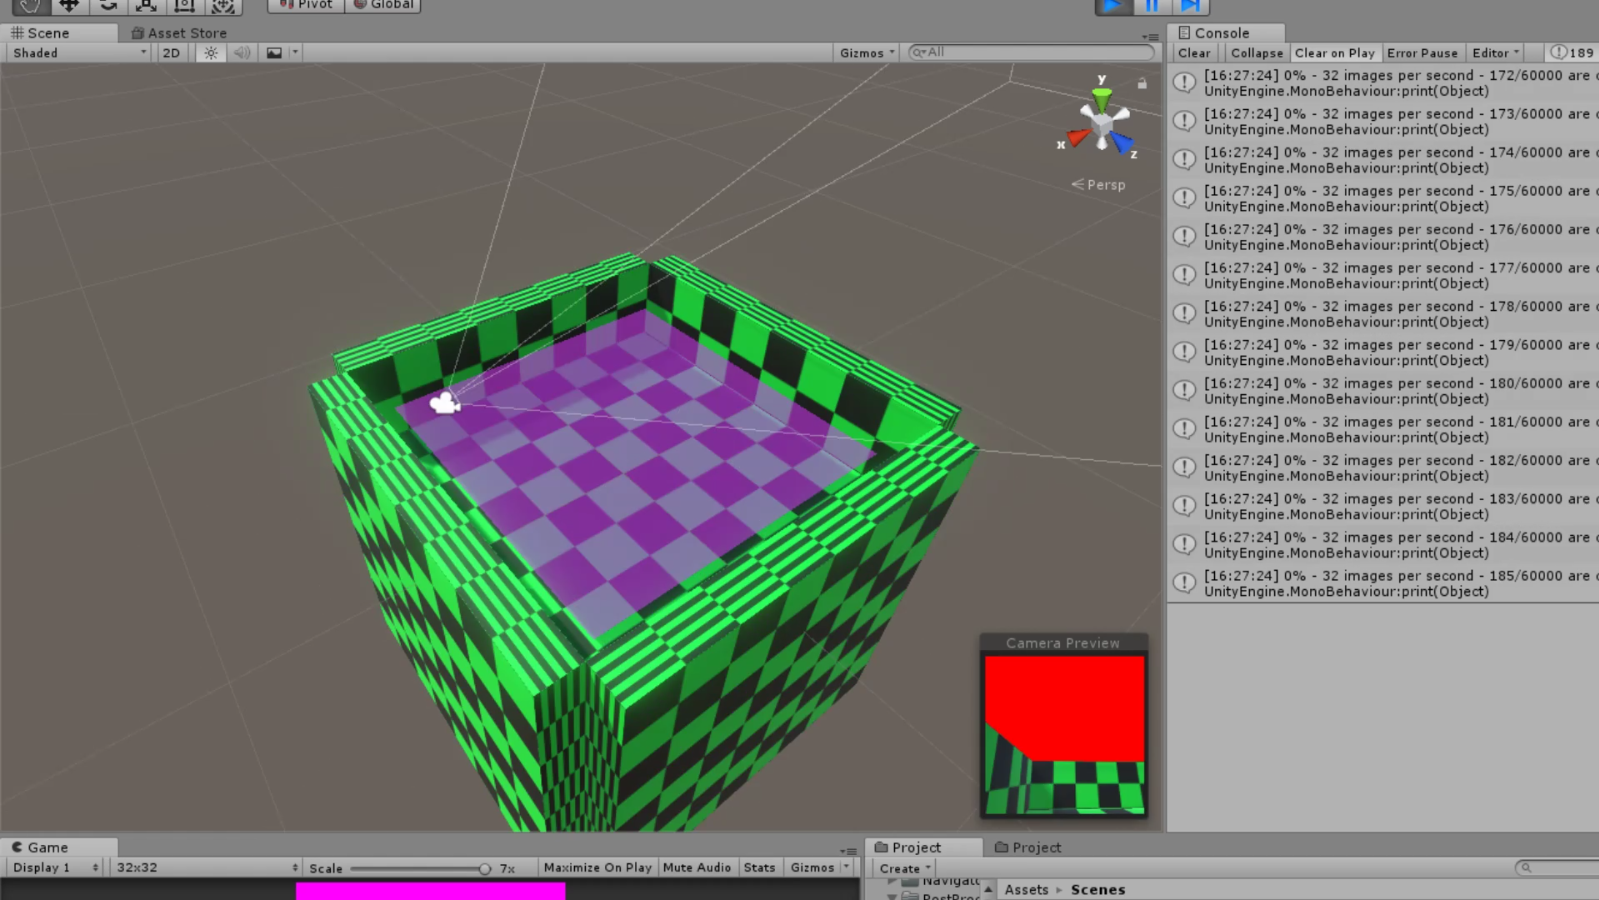
\includegraphics[width=\imgWidth]{images/workflow/Functional1.png} \\[\picVdist]
  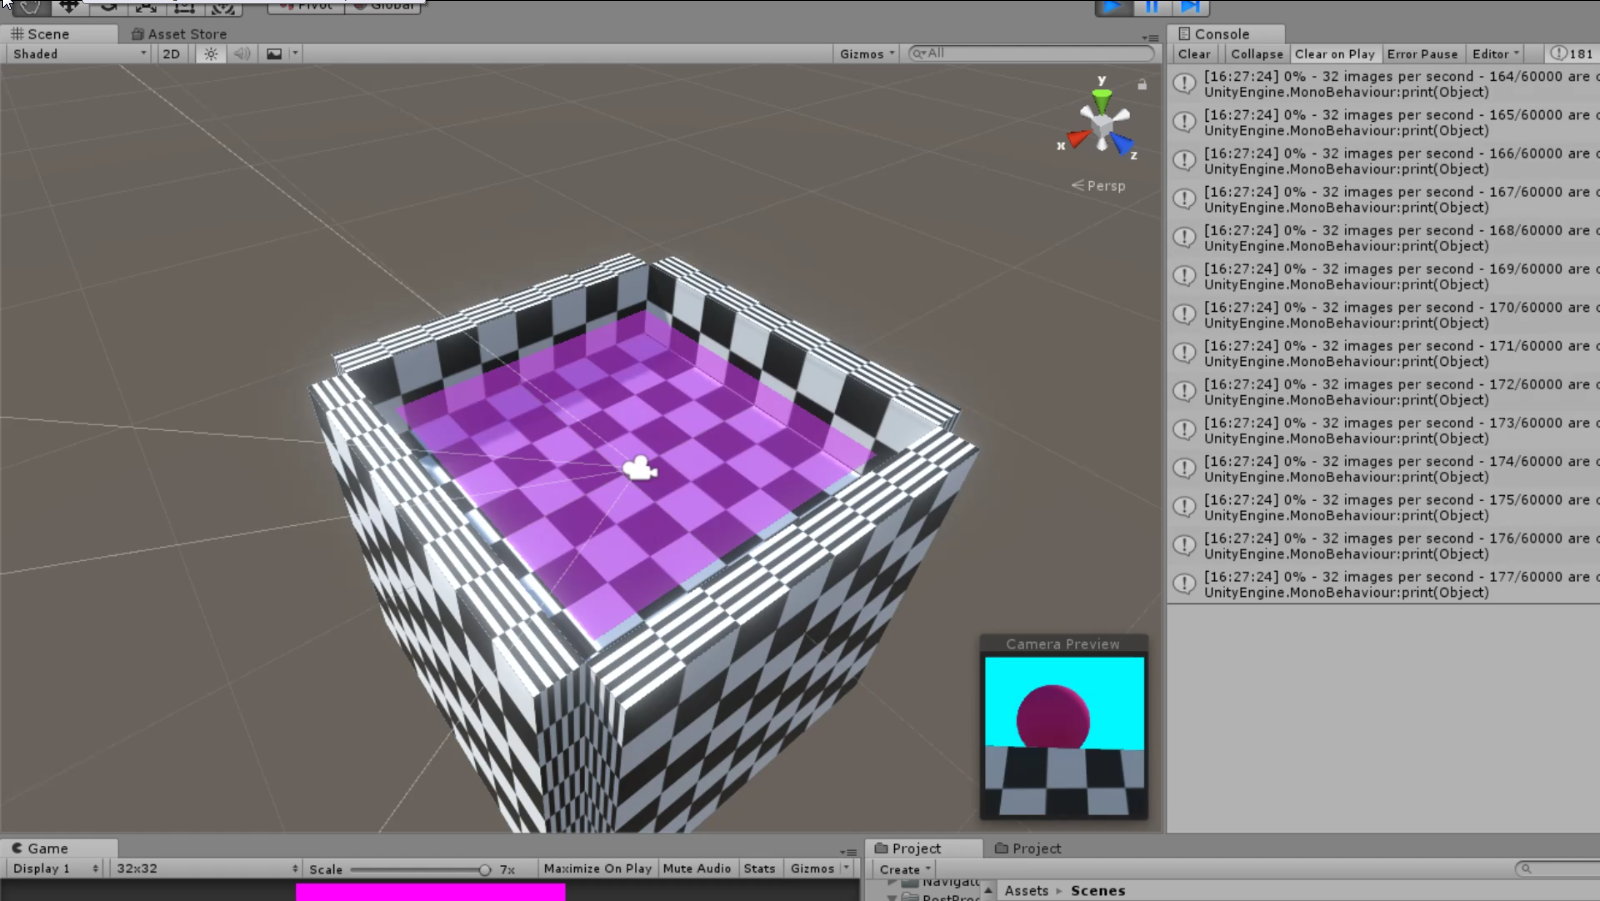
\includegraphics[width=\imgWidth]{images/workflow/Functional2.png}
  \caption{Training data is being captured in the functional prototype level.}
  \label{FunctionalCapture}
  \figsource{own graphic}
\end{figure}

\section{Top down}
This prototype was used to evaluate the suitability of the network for a top town game. In this prototype the player has to go from one colored platform to another while avoiding the red walls. The challenge should be created by only training the network on data that is captured by pointing the camera at one of the colored platforms. Training the network on this data resulted only in making the network output blurry, when the player was not positioned on a platform (\cref{WalkOffPlatform} and \cref{TopDownUnity}). Because the prototype did not present an interesting direction, it was abandoned.

\begin{figure}[p]
  \centering
  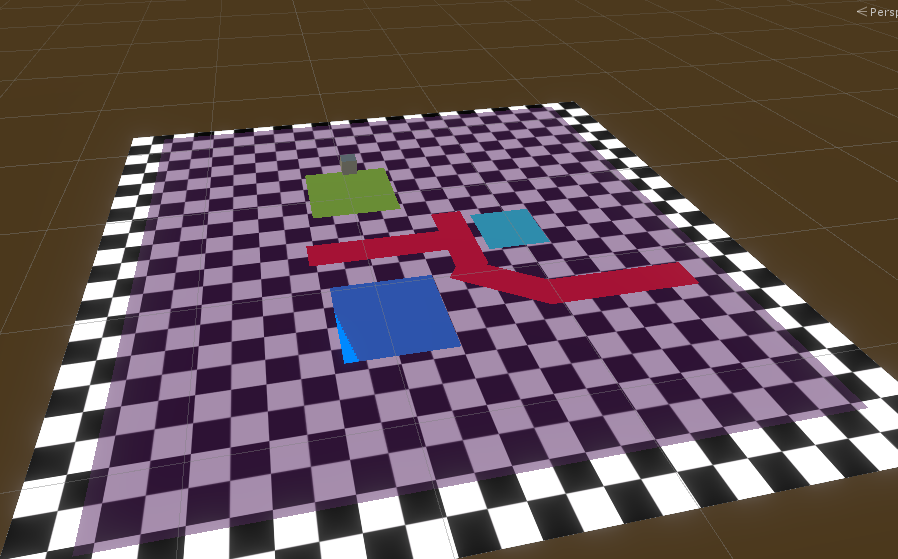
\includegraphics[width=\imgWidth]{images/workflow/TopDownLevel.png}
  \caption{Top down prototype level as seen in the editor}
  \label{TopDownUnity}
  \figsource{own graphic}
\end{figure}

\begin{figure}[p]
  \centering
  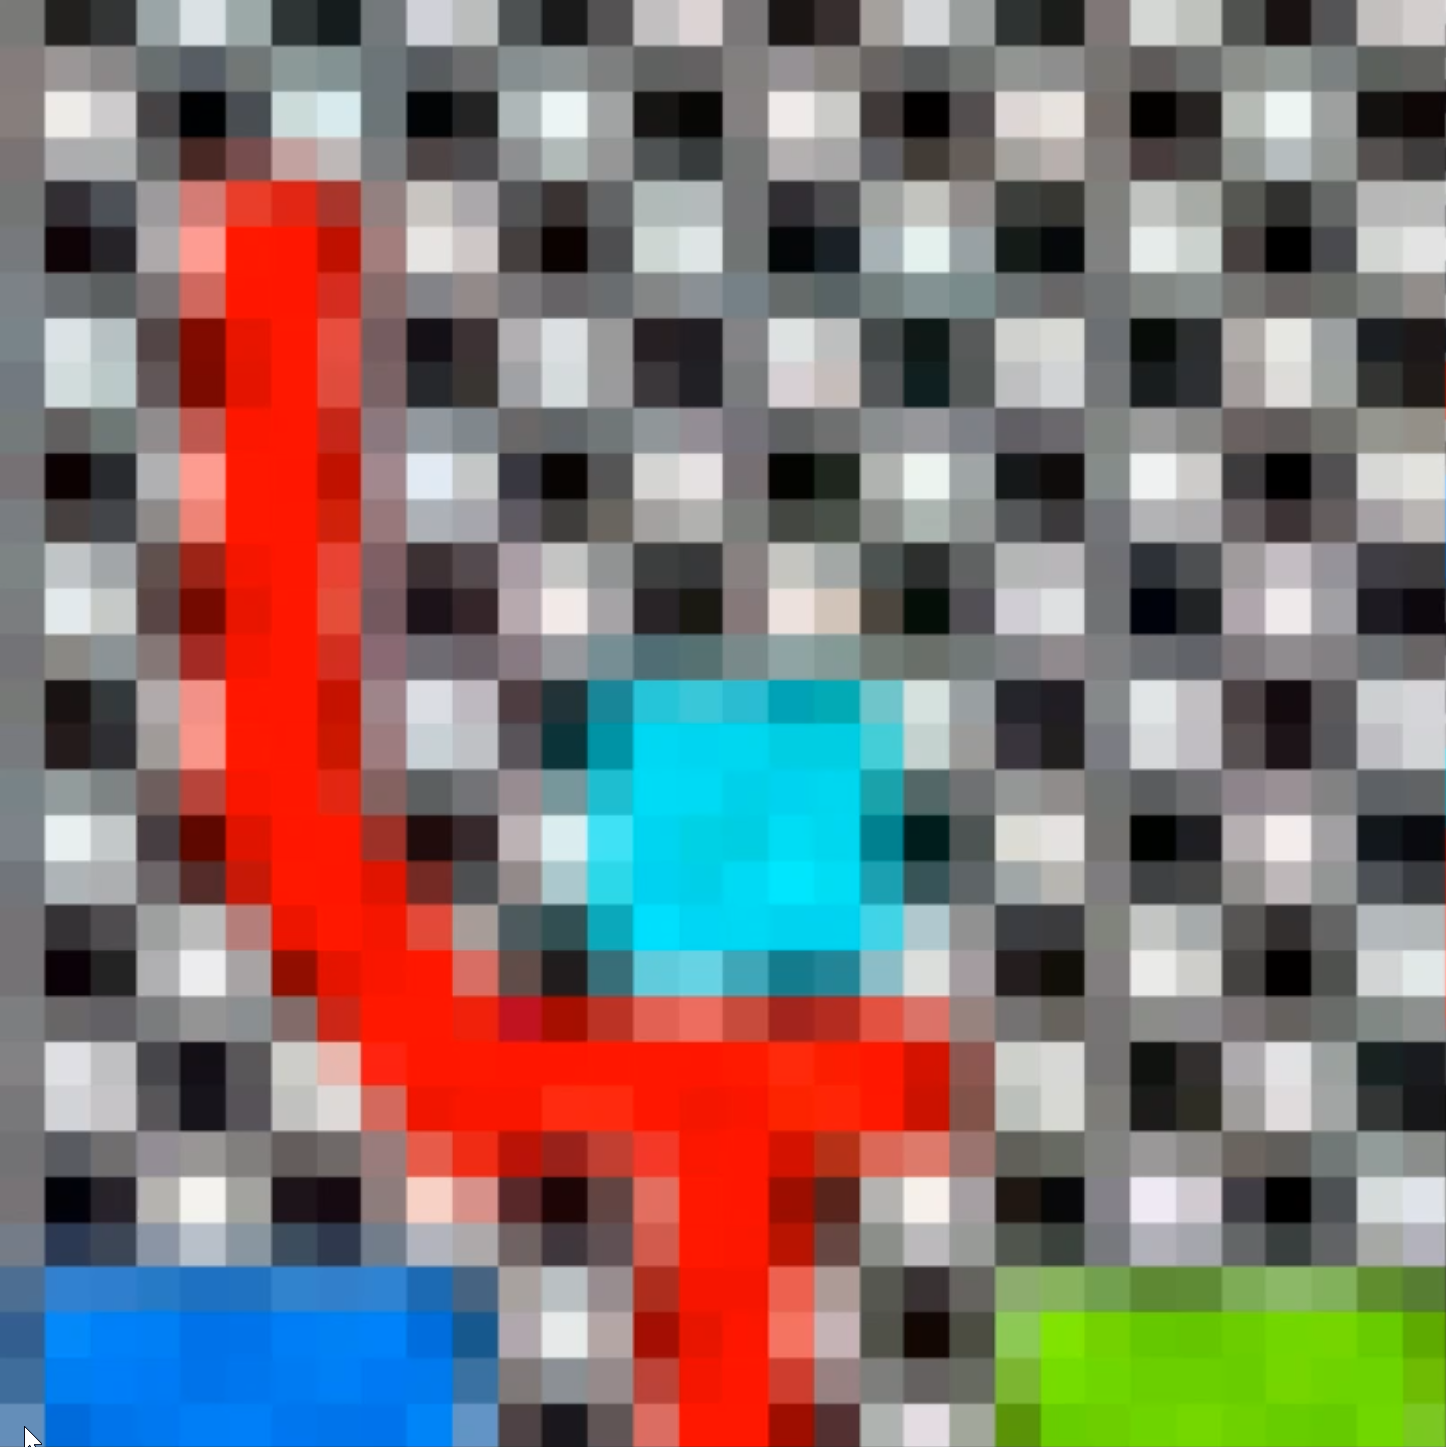
\includegraphics[width=\imgWidth]{images/workflow/TopDownOn.png} \\[\picVdist]
  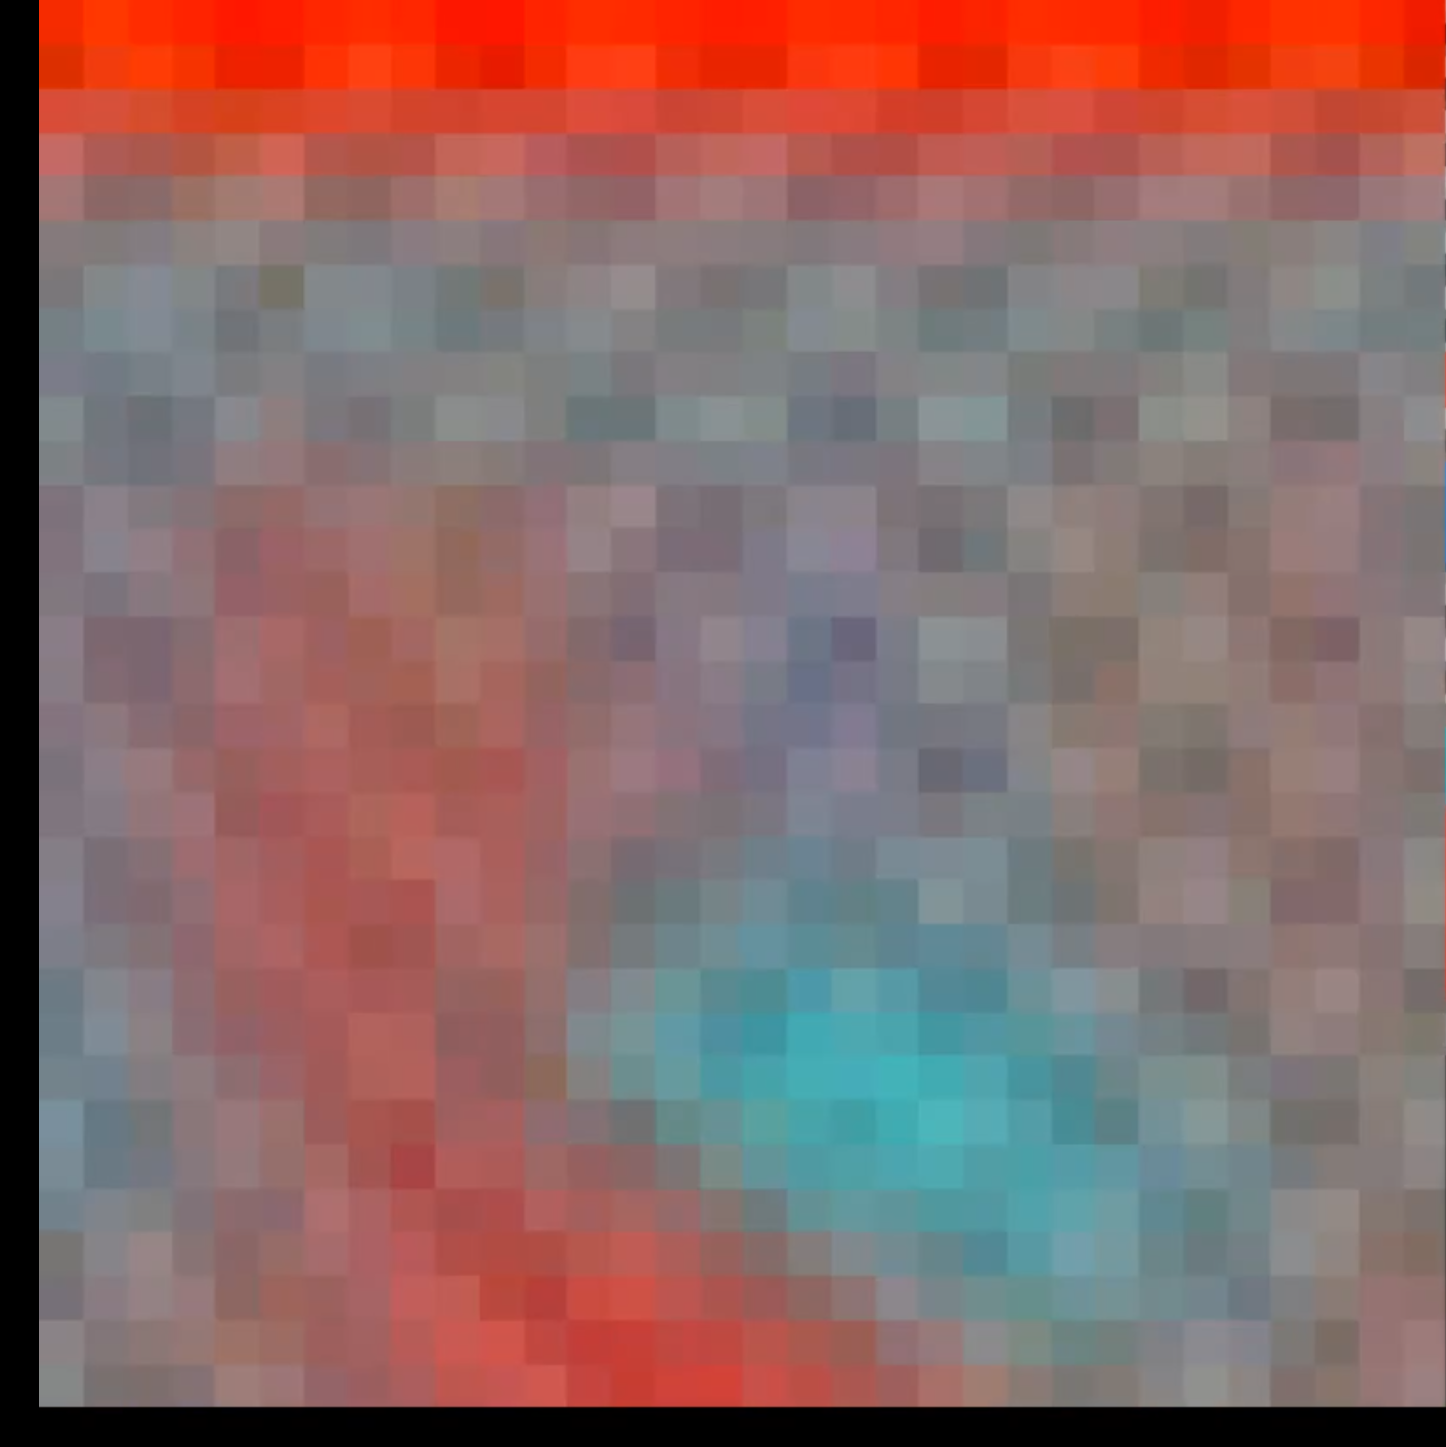
\includegraphics[width=\imgWidth]{images/workflow/TopDownOff.png}
  \caption{In the top down prototype, the network output gets blurry when the player walks off a platform.}
  \label{WalkOffPlatform}
  \figsource{own graphic}
\end{figure}


\section{Walking sim}
Here the idea was to present the level to the player through the neural network to create an interesting visual appearance. I also experimented with having certain objects only be visible if the player is at a certain position in the environment (\cref{WalkingSim}). This idea was further explored in the next prototype.

\begin{figure}[p]
  \centering
  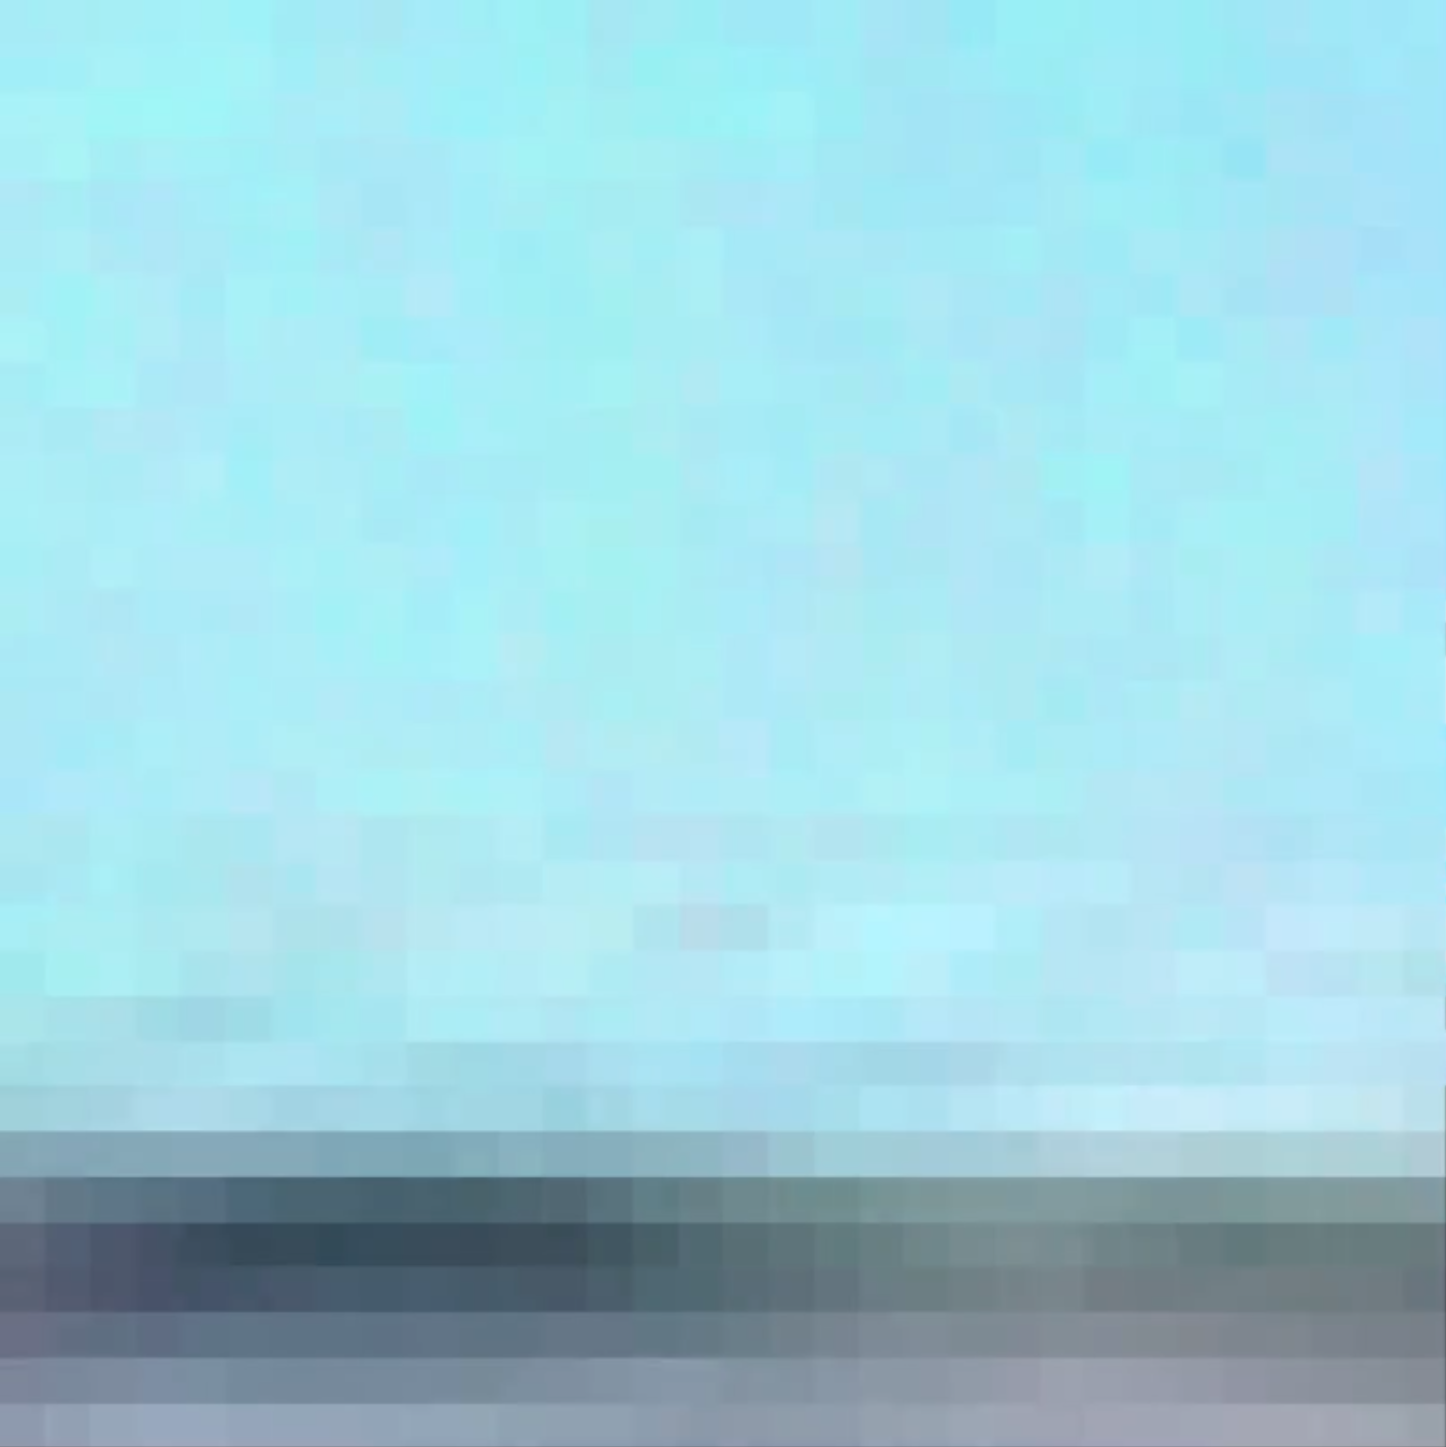
\includegraphics[width=\imgWidth]{images/workflow/WalkingSimNothing.png} \\[\picVdist]
  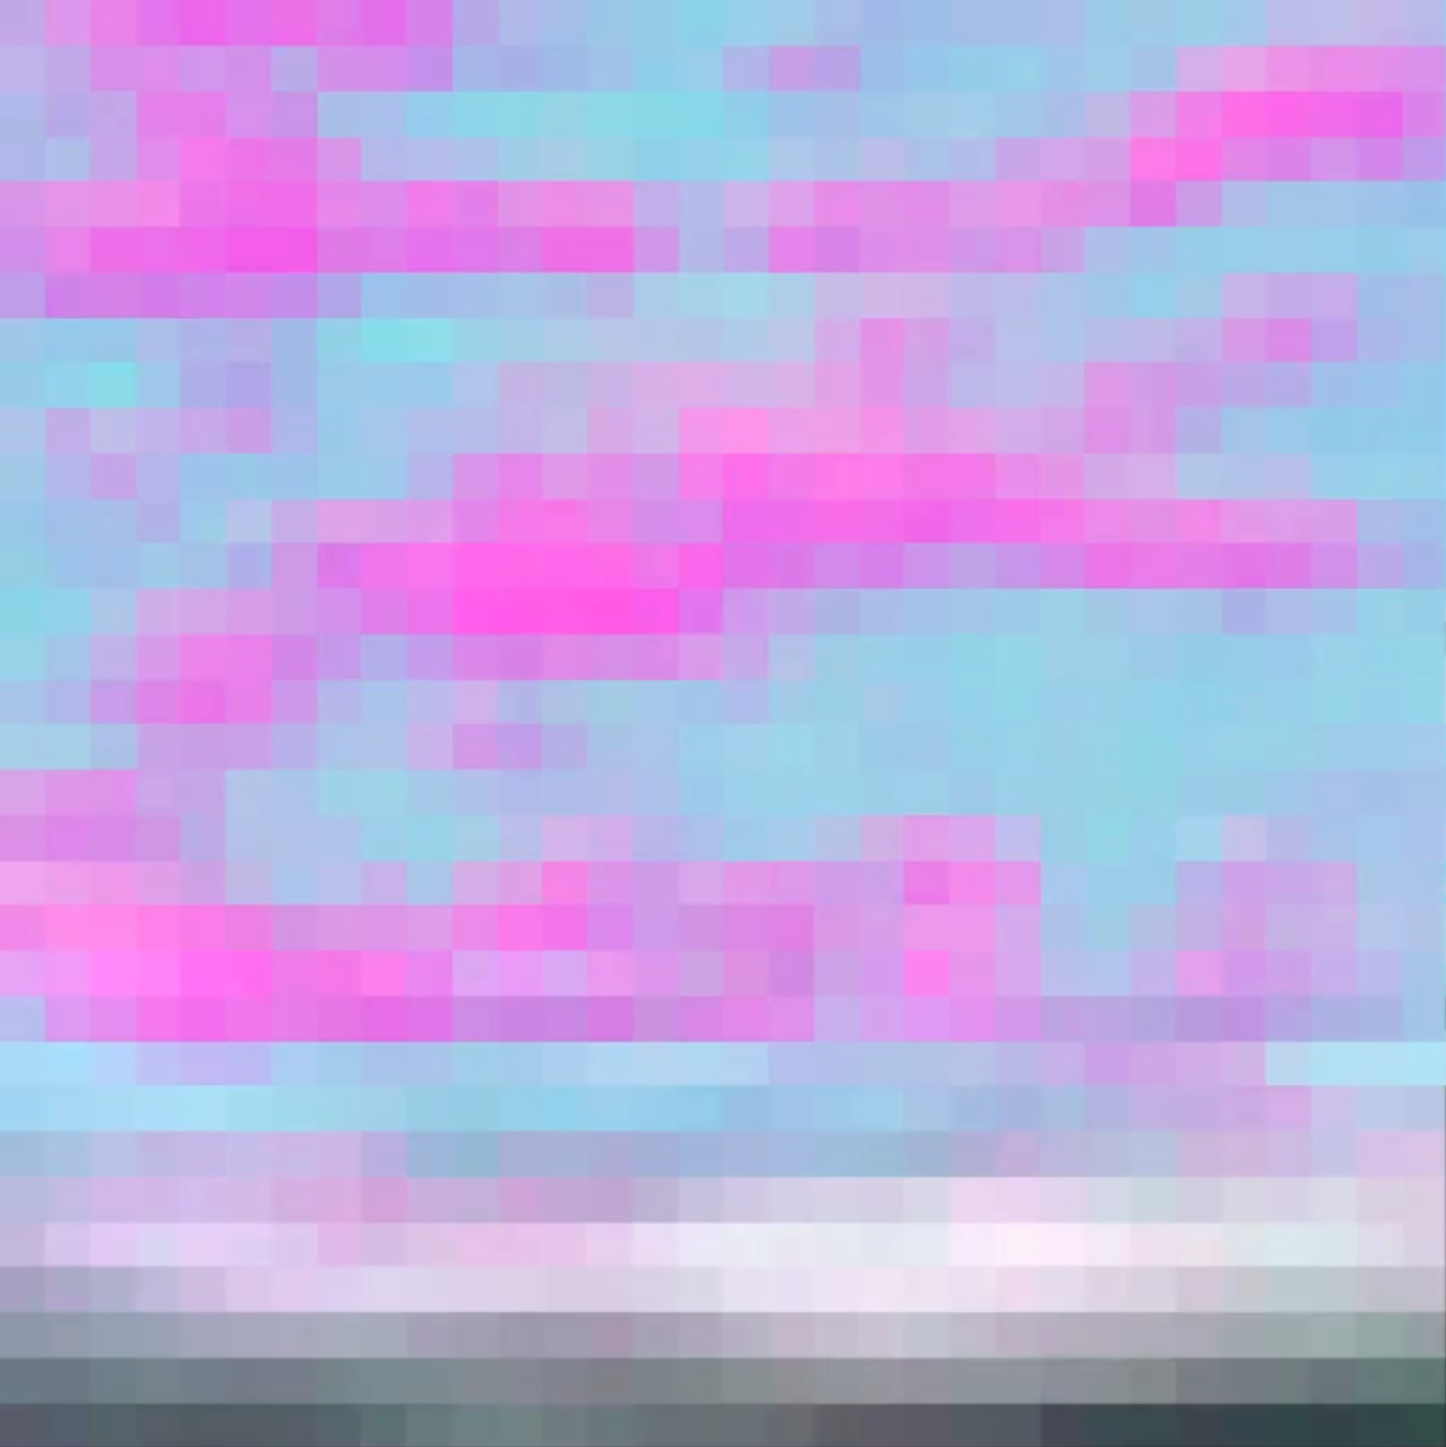
\includegraphics[width=\imgWidth]{images/workflow/WalkingSimCloud.png}
  \caption{Objects can only be seen, when the player stands at certain locations}
  \label{WalkingSim}
  \figsource{own graphic}
\end{figure}


\section{Object morphing}
This prototype has a level that is divided into four differently colored platforms (\cref{MorphingLevel}) that are surrounded by tall pillars. The coloring of the platforms and the pillars help the player to orient himself. In the center four different objects are placed (\cref{MorphingObjs}). Each of the objects is linked with a different marker group as described in \cref{DataGeneration}. The marker groups are shown in \cref{MorphingMarkers}. There is a marker placed on top of each platform. This means that if an observation is taken from a specific platform only one of the four objects is displayed in the center. When the player crosses from one platform to another the center object is morphed from one object to another as seen in \cref{MorphingToOther}. This is probably because a neural network with a limited amount of parameters cannot model an instantaneous change in "pixel space".

\begin{figure}[p]
  \centering
  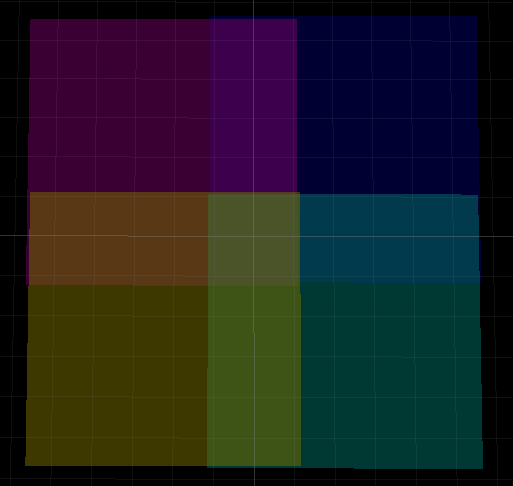
\includegraphics[width=\imgWidth]{images/workflow/object_morphing/CaptureAreas.png}
  \caption{These are the 4 markers (explained in \cref{DataGeneration}) of the morphing environment. Overlapping areas are differently colored.}
  \label{MorphingMarkers}
  \figsource{own graphic}
\end{figure}

\begin{figure}[p]
  \centering
  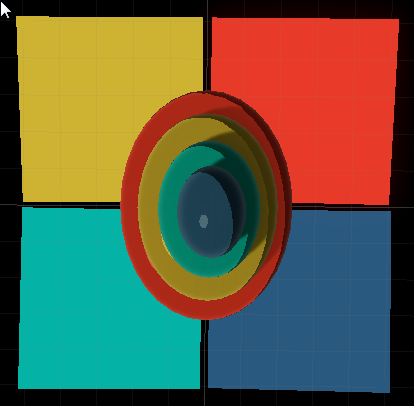
\includegraphics[width=\imgWidth]{images/workflow/object_morphing/TopDown.png}
  \caption{Top down view of the level with only one object activated in the middle}
  \label{MorphingLevel}
  \figsource{own graphic}
\end{figure}

\begin{figure}[p]
  \centering
  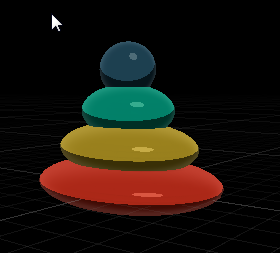
\includegraphics[width=0.49\textwidth, height=0.49\textwidth]{images/workflow/object_morphing/Obj_1.png}
  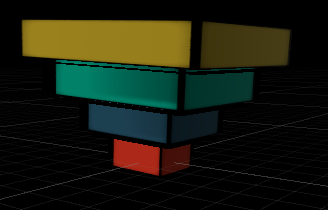
\includegraphics[width=0.49\textwidth, height=0.49\textwidth]{images/workflow/object_morphing/Obj_2.png} \\[\picVdist]
  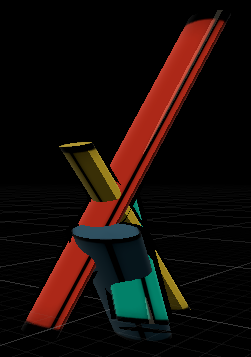
\includegraphics[width=0.49\textwidth, height=1\textwidth]{images/workflow/object_morphing/Obj_3.png}
  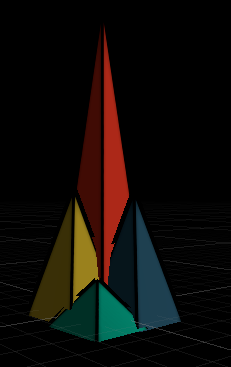
\includegraphics[width=0.49\textwidth, height=1\textwidth]{images/workflow/object_morphing/Obj_4.png}
  \caption{The 4 differnt objects in the center of the level}
  \label{MorphingObjs}
  \figsource{own graphic}
\end{figure}

\begin{figure}[p]
  \centering
  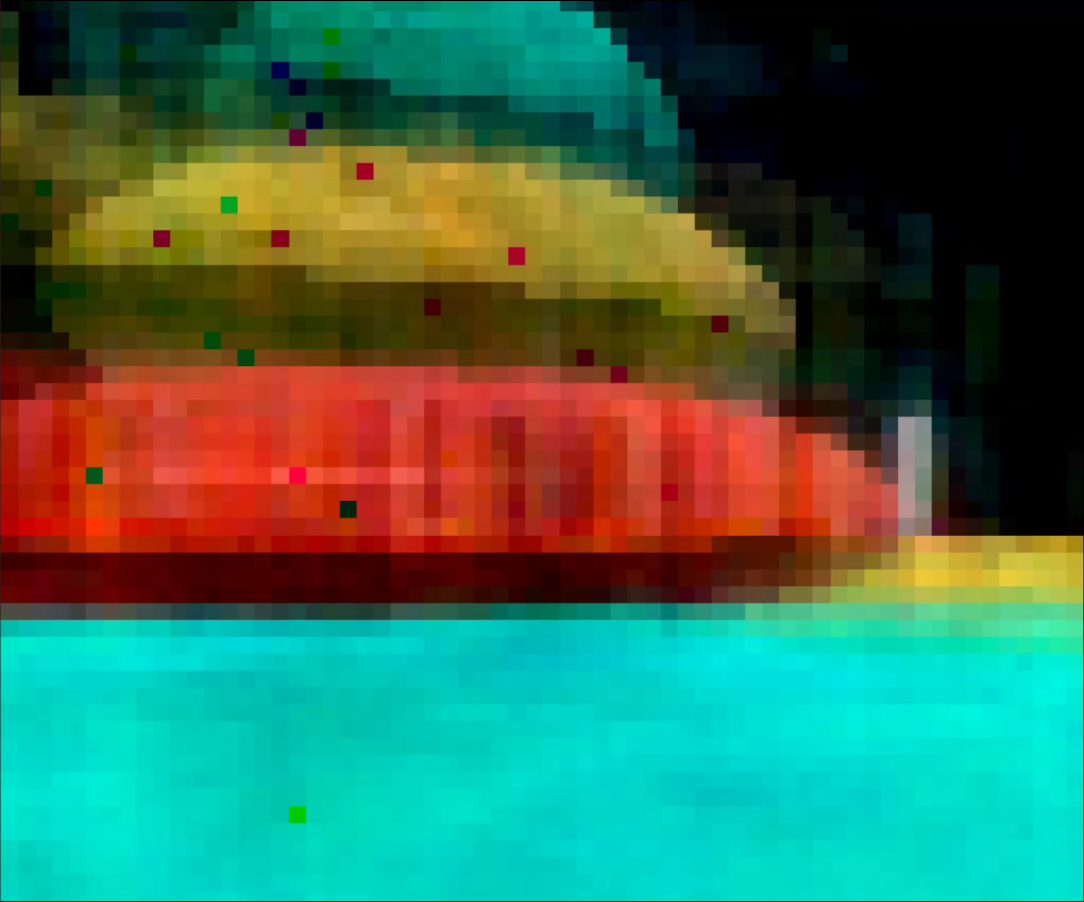
\includegraphics[width=\imgWithTripple, width=\imgWithTripple]{images/workflow/object_morphing/Morph1.png} \\[\picVdist]
  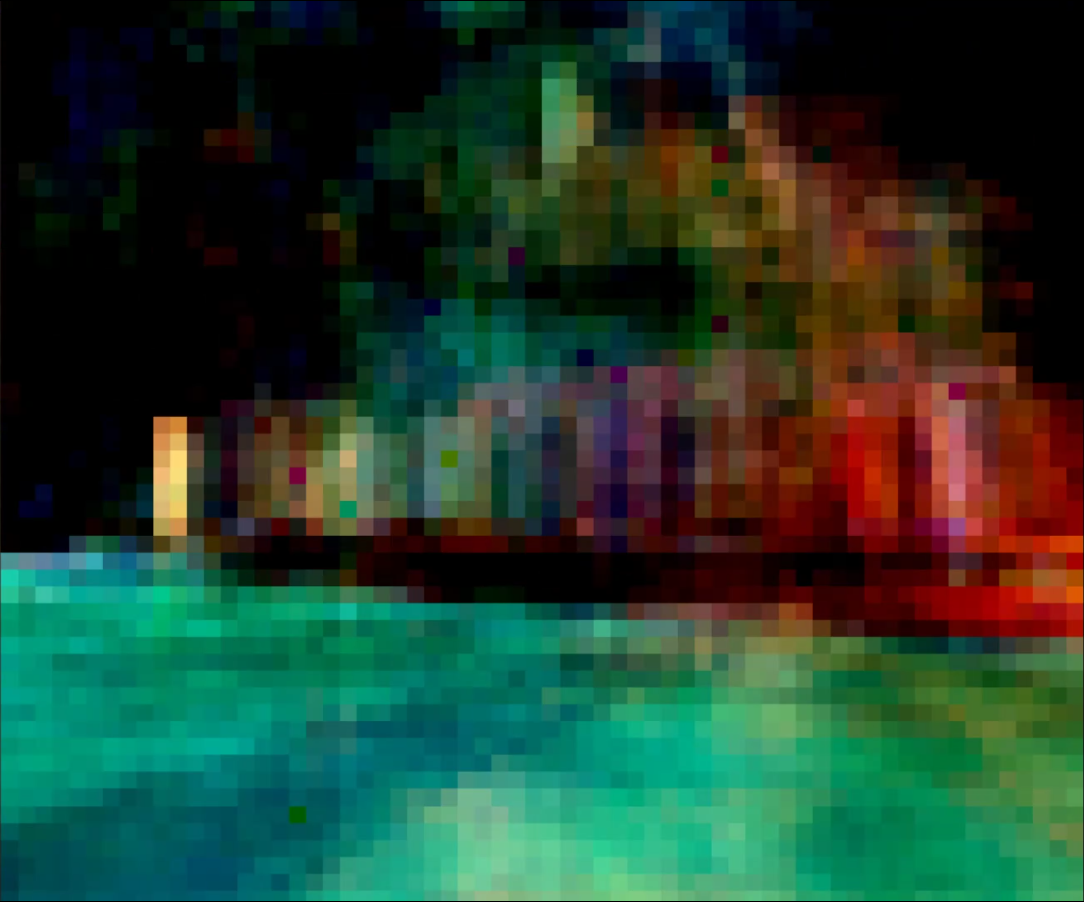
\includegraphics[width=\imgWithTripple, width=\imgWithTripple]{images/workflow/object_morphing/Morph2.png} \\[\picVdist]
  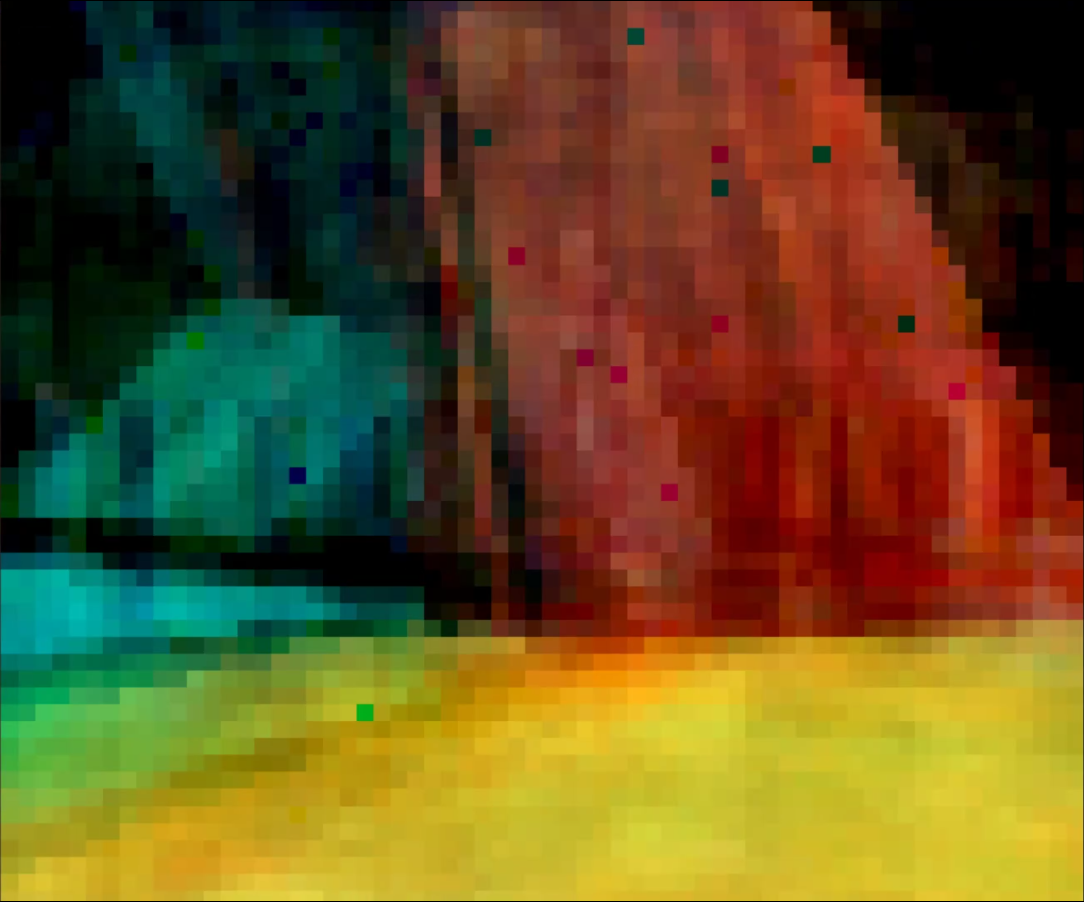
\includegraphics[width=\imgWithTripple, width=\imgWithTripple]{images/workflow/object_morphing/Morph4.png}
  \caption{The center object morphs into a different object when the player crosses from one marker into another.}
  \label{MorphingToOther}
  \figsource{own graphic}
\end{figure}
